\documentclass{article}
\usepackage{graphicx}

\usepackage{tikz}
\usetikzlibrary{arrows}

\usepackage[utf8]{inputenc}
\usepackage[a4paper]{geometry}
%\usepackage{fullpage}
\usepackage{etoolbox}
\usepackage{amsmath}
\usepackage{latexsym}
\usepackage{booktabs}
\usepackage{adjustbox}


\makeatletter
\patchcmd{\maketitle}{\@fnsymbol}{\@alph}{}{}  % Footnote numbers from symbols to small letters
\makeatother

\title{Huiswerk 1\\ \large{Statistisch Redeneren UvA-2015}}
\author{Jelte Fennema\thanks{Student nummer 10183159} ~\& Bas van den
Heuvel\thanks{Student nummer 10343725}}

\date{\today}

\begin{document}
\maketitle

\begin{enumerate}
    \item
        \begin{enumerate}
            \item
                $U = \{1,2,3,4,5,6\}$, dit is niet een unieke mogelijkheid. Er
                zijn ook andere uitkomstenruimten bedenkbaar.

            \item
                \begin{align*}
                    A &= \{1,2,3,4,5,6\}\\
                    U&=A \times A
                \end{align*}

            \item
                $P((6,6)) = \frac16 \cdot \frac16 = \frac1{36}$

            \item
                De uitkomsten set waarbij geldt dat het totaal van de ogen 9 is
                is $B$.

                \begin{align*}
                    B &= \{(3,6), (6,3), (5,4), (4,5)\}\\
                    P(B)&= 4\cdot\frac1{36}=\frac19
                \end{align*}

            \item
                \begin{align*}
                    C &= \{(a, b) | a \in A, b \in A, a+b = n\}\\
                    P(C)&= |C| \cdot \frac1{36}
                \end{align*}

            \item De situaties waarbij een even aantal ogen wordt gegooid zijn
                de situaties waarbij 2 maal een even aantal ogen is gegooid of 2
                maal een oneven aantal ogen. Aangezien er evenveel even als
                oneven ogen zijn kan je een van de twee berekenen en dat
                vertweevoudigen. Er zijn 3 mogelijkheden om even te gooien bij
                elke worp, dus er zijn 9 mogelijkheden om twee maal even te
                gooien. $D$ is de set waarbij het totaal aantal gegooide ogen even
                is.
                $$
                P(D) = 9 \cdot \frac1{36} \cdot 2 = \frac12
                $$

        \end{enumerate}

    \item
        \begin{align*}
            P(1) &= P(U) - P(A\cup B) = 1 - 0.8 = 0.2\\
            P(A\cup B) &= P(A) + P(B) + P(A \cap B)\\
            P(3) &= P(A\cap B) \\
                 &= P(A) + P(B) + P(A\cup B)\\
                 &= 0.5 + 0.7 - 0.8 = 0.4\\
            P(2) &= P(A) - P(3) = 0.5 - 0.4 = 0.1\\
            P(4) &= P(B) - P(3) = 0.7 - 0.4 = 0.3
        \end{align*}

    \item
        \begin{enumerate}
            \item
                \begin{minipage}[t]{\linewidth}
                    \adjustbox{valign=t}{
                        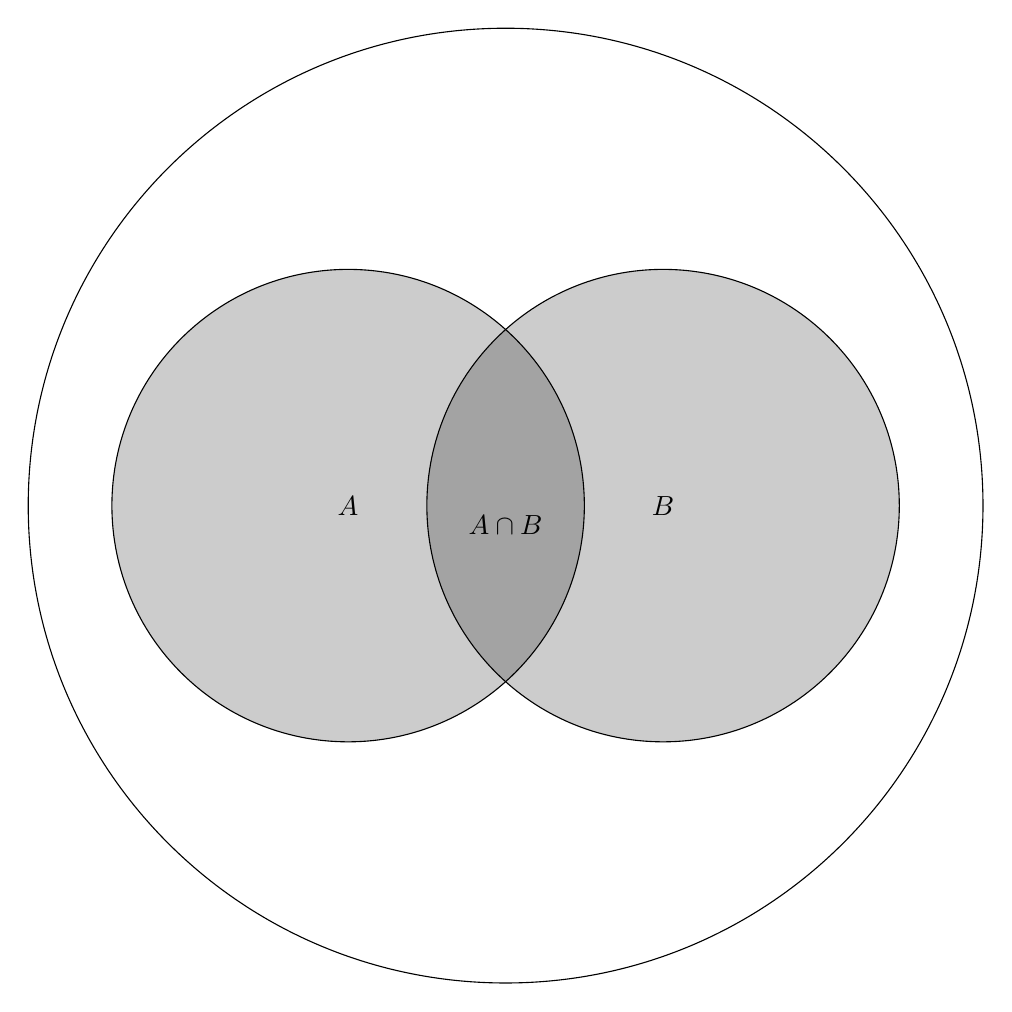
\begin{tikzpicture}
                            \tikzset{venn circle/.style={draw,circle,minimum
                            width=6cm,fill=#1, fill opacity=0.2, text opacity=1}}
                            \tikzset{universe/.style={draw,circle,minimum
                            width=\linewidth}}

                            \node [venn circle] (A) at (0,0) {$A$};
                            \node [venn circle] (B) at (0:4cm) {$B$};
                            \node [universe] (U) at (0:2cm) {};
                            \node[below] at (barycentric cs:A=1/2,B=1/2 ) {$A \cap B$};
                        \end{tikzpicture}
                    }
                \end{minipage}
                Zoals te zien is in het venn diagram hierboven, wordt de kans op
                $A\cap B$ dubbel geteld als je de kans van $A$ en $B$ bij elkaar
                op telt. Dus om de kans op $A\cup B$ te krijgen moet je de kans
                daarop een maal vanaf trekken.
                Om algebraisch te bewijzen hebben we eerst de kansaxioma's
                nodig.
                \begin{align}
                    P(A) &\ge 0\\
                    P(U) &= 1 \\
                    A,B \subset U, A\cap B =\emptyset : P(A\cup B) &= P(A)+P(B)
                \end{align}

                Dan nu het bewijs:
                \begin{align}
                    B' &= B\setminus A & (definitie)\\
                    A \cap B' &= \emptyset & (4, verzamelingenleer)\\
                    A \cup B &= A \cup B' & (4, verzamelingenleer)\\
                    P(A\cup B) &= P(A) + P(B') & (3, 5, 6)\\
                    B' \cap (A \cap B) &= \emptyset & (4, verzamelingenleer)\\
                    B' \cup (A\cap B) &= B & (4, verzamelingenleer)\\
                    P(B') + P(A \cap B) &= P(B) & (3, 8, 9)\\
                    P(B') &= P(B) - P(A\cap B) & (10)\\
                    P(A\cup B) &= P(A) + P(B) - P(A\cap B) & (7, 11)
                \end{align}
                $\Box$

            \item
                \begin{align}
                    \lnot A \cap A &= \emptyset & (verzamelingenleer)\\
                    P(\lnot A \cup A) &= P(\lnot A) + P(A) & (3, 13)\\
                    \lnot A &= U\setminus A & (verzamelingenleer)\\
                    \lnot A \cup A &= U & (15, verzamelingenleer)\\
                    P(U) &= P(\lnot A) + P(A) & (14, 16)\\
                         &= 1 & (17, 2)\\
                    P(\lnot A) &= 1 - P(A) & (17, 18)
                \end{align}
                $\Box$

            \item
                \begin{align}
                    \lnot B \cap B &= \emptyset & (verzamelingenleer)\\
                    A\cap B &\subseteq B & (verzamelingenleer)\\
                    A\cap \lnot B &\subseteq \lnot B & (verzamelingenleer)\\
                    (A\cap B) \cap (A \cap \lnot B) &= \emptyset  &(20, 21, 22,
                    verzamelingenleer)\\
                    \lnot B &= U\setminus B & (verzamelingenleer)\\
                    A\cap \lnot B &= A \cap (U\setminus B) & (24)\\
                    A &\subseteq U & (verzamelingenleer)\\
                    A\cap \lnot B &= A \setminus B & (26)\\
                    (A\setminus B) \cap (A\cap B) &= A & (verzamelingenleer)\\
                    (A\cap B) \cup (A \cap \lnot B) &=A & (27, 28)\\
                    P(A\cap B) + P(A \cap \lnot B) &= P(A) & (3, 29, 23)
                \end{align}
                $\Box$

            \item
                \begin{align}
                    A \cap U &= A & (verzamelingenleer)\\
                    \bigcup_{i=1}^n B_i &= U & (gegeven)\\
                    A \cap \bigcup_{i=1}^n B_i &= A & (31, 32)\\
                    \bigcup_{i=1}^n A \cap B_i &= A & (33, verzamelingenleer)\\
                    A \cap B_i &\subseteq B_i & (verzamelingenleer)
                \end{align}

                Omdat alle $B_i$ disjunct zijn, en $A \cap B_i \subseteq B_i$,
                zijn ook alle $A \cap B_i$ disjunct.

                \begin{align}
                    P(A) &= \sum_{i=1}^n P(A \cap B_i) & (34, 35)
                \end{align}
                $\Box$

        \end{enumerate}

    \item
        \begin{align}
            P(A|B) &= \frac{P(A \cap B)}{P(B)} & (conditionele\:kans)\\
            P(B|A) &= \frac{P(B \cap A)}{P(A)} & (conditionele\:kans)\\
            P(A \cap B) &= P(A) \cdot P(B|A) & (38)\\
            P(A|B) &= \frac{P(A)}{P(B)} \cdot P(B|A) & (37, 39)
        \end{align}
        $\Box$

    \item
        \begin{enumerate}
            \item
                De oppervlakte van $B$ wordt de nieuw $U$, door te normaliseren.

            \item
                Als je het universum terugbrengt naar $B$, wil je daarna verder
                kunnen rekenen met de axioma's. Stel $B'$ is de genormaliseerde
                $B$, dan geldt $P(B')=1$. In de conditionele kans normaliseer je
                alle kansberekeningen naar het oppervlak van $B$.

        \end{enumerate}

    \item
        \begin{enumerate}
            \item
                Base case:

                \begin{align}
                    n &= 2 &\\
                    P(A_1 A_2) &= P(A_1 | A_2) P(A_2) & (conditionele\:kans)
                \end{align}

                Inductie stap:

                \begin{align}
                    P(A_1 A_2 \cdots A_n) &= P(A_n \cdots A_2 A_1) &
                    (verzamelingenleer) \\
                    P(A_n \cdots A_2 A_1) &= P(A_n | A_1 A_2 \cdots A_{n-1})
                    \cdots P(A_2 | A_1) P(A_1) & (aanname) \\
                    P(A_{n+1} A_n \cdots A_2 A_1) &= P(A_{n+1} | A_1 A_2 \cdots
                    A_n) P(A_n \cdots A_2 A_1) & (conditionele\:kans) \\
                    &= P(A_{n+1} | A_1 A_2 \cdots A_n) P(A_n | A_1 A_2 \cdots
                    A_{n-1}) & \notag \\
                             & \cdots P(A_2 | A_1) P(A_1) & (44)
                \end{align}
                $\Box$

            \item
                Nee, bij (a) hebben we al een andere mogelijkheid gebruikt bij
                het bewijs.

        \end{enumerate}

    \item
        \begin{enumerate}
            \item
            \item
                Conditionele kans.

        \end{enumerate}

    \item
        \begin{enumerate}
            \item
                \begin{align}
                    A \perp B \to P(A \cap B) &= P(A) P(B) & (onafhankelijk) \notag \\
                                              &= P(A) (1 - P(\lnot B)) & (complement)
                    \notag \\
                                              &= P(A) -P(A)P(\lnot B) \\
                    P(A \cap B) &= P(A) + P(B) - P(A \cup B) \notag \\
                    P(A) - P(A) P(\lnot B) &= P(A) + P(B) - P(A \cup B) & (47) \\
                    -P(A) P(\lnot B) &= P(B) - P(A \cup B) \notag \\
                    P(A) P(\lnot B) &= P(A \cup B) - P(B) \notag \\
                                    &= P(A) + P(B) - P(A \cap B) - P(B) \notag \\
                                    &= P(A) - P(A \cap B) \notag \\
                                    &= P(A \cap B) + P(A \cap \lnot B) - P(A \cap B)
                    & (30) \notag \\
                    &= P(A \cap \lnot B) \to A \perp \lnot B
                \end{align}
                $\Box$

            \item
                Vervang A voor B en B voor A in bovenstaand bewijs, dan geldt
                $P(\lnot A \cap B) = P(\lnot A) P(B) \to \lnot A \perp B$.

            \item
                Door een van de twee regels hierboven toe te passen, en het
                vervolgens te herhalen met de volgende, geldt ook $P(\lnot A
                \cap \lnot B) = P(\lnot A) P(\lnot B) \to \lnot A \perp \lnot
                B$.

        \end{enumerate}

    \item
        \newcommand{\kw}{\mathrm{w}}
        \newcommand{\kr}{\mathrm{r}}
        \newcommand{\I}{\mathrm{I}}
        \newcommand{\II}{\mathrm{II}}
        \newcommand{\III}{\mathrm{III}}

        \begin{align*}
            P(K = \kw) &= P(K = \kw | V = \I) + P(K = \kw | V = \II) +
            P(K = \kw | V = \III) \\
            &= \frac5{18} + \frac29 + \frac16 = \frac23 \\
            P(K = \kr) &= P(K = \kr | V = \I) + P(K = \kr | V = \II) +
            P(K = \kr | V = \III) \\
            &= \frac1{18} + \frac19 + \frac16 = \frac13 \\ \\
            P(V = \I | K = \kw) &= \frac{P(V = \I)}{P(K = \kw)} \cdot
            P(K = \kw | V = \I) \\
            &= \frac13 \cdot \frac32 \cdot \frac5{18} = \frac{15}{36} \\
            P(V = \II | K = \kw) &= \frac13 \cdot \frac32 \cdot \frac29
            = \frac13 \\
            P(V = \III | K = \kw) &= \frac13 \cdot \frac32 \cdot \frac16
            = \frac14 \\
            P(V = \I | K = \kr) &= \frac13 \cdot \frac31 \cdot \frac1{18} =
            \frac1{18} \\
            P(V = \II | K = \kr) &= \frac19 \\
            P(V = \III | K = \kr) &= \frac16 \\
        \end{align*}

\end{enumerate}


\end{document}
